\documentclass[11pt]{article}

\usepackage[margin=1in]{geometry}
\usepackage{amsmath, amssymb, amsthm}
\usepackage{enumitem}
\usepackage{tikz}
\usetikzlibrary{arrows.meta, positioning, fit, shapes.geometric}

\newcommand{\Z}{\mathbb{Z}}
\newcommand{\R}{\mathbb{R}}
\newcommand{\N}{\mathbb{N}}

\pagestyle{empty}

\begin{document}

\begin{center}
  {\Large\bfseries Weekly Assignment: Functions (Epp Ch.\ 7)}
\end{center}

\bigskip

\noindent
Complete each of the following problems.  Show all work and justify your answers.

\bigskip

%% ─────────────────────────────────────────────
\noindent\textbf{Problem 1} (Epp 7.1 \#2). \;
Let $X = \{1, 3, 5\}$ and $Y = \{a, b, c, d\}$.
Define $g \colon X \to Y$ by the following arrow diagram.

\begin{center}
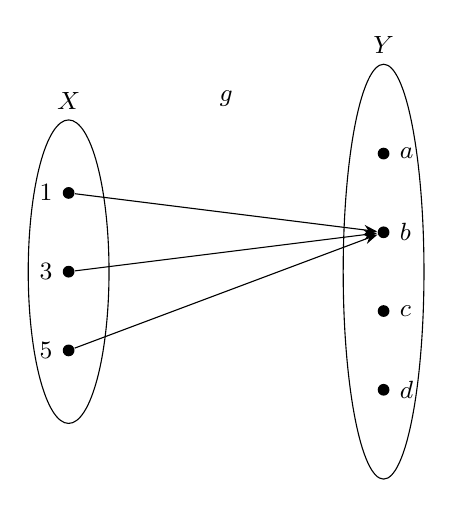
\begin{tikzpicture}[
    >=Stealth,
    dot/.style={circle, fill, inner sep=1.5pt},
    every node/.style={font=\small}
  ]
  % Domain
  \node[dot, label=left:{$1$}] (x1) at (0,2)   {};
  \node[dot, label=left:{$3$}] (x3) at (0,1)   {};
  \node[dot, label=left:{$5$}] (x5) at (0,0)   {};
  \node[draw, ellipse, fit=(x1)(x3)(x5), inner sep=8pt, label=above:{$X$}] {};

  % Codomain
  \node[dot, label=right:{$a$}] (a) at (4,2.5) {};
  \node[dot, label=right:{$b$}] (b) at (4,1.5) {};
  \node[dot, label=right:{$c$}] (c) at (4,0.5) {};
  \node[dot, label=right:{$d$}] (d) at (4,-0.5){};
  \node[draw, ellipse, fit=(a)(b)(c)(d), inner sep=8pt, label=above:{$Y$}] {};

  % Arrows
  \draw[->] (x1) -- (b);
  \draw[->] (x3) -- (b);
  \draw[->] (x5) -- (b);

  % Label
  \node at (2,3.2) {$g$};
\end{tikzpicture}
\end{center}

\begin{enumerate}[label=\alph*.]
  \item Write the domain of $g$ and the co-domain of $g$.
  \item Find $g(1)$, $g(3)$, and $g(5)$.
  \item What is the range of $g$?
  \item Is $3$ an inverse image of $a$? Is $1$ an inverse image of $b$?
  \item What is the inverse image of $b$? Of $c$?
  \item Represent $g$ as a set of ordered pairs.
\end{enumerate}

\bigskip

%% ─────────────────────────────────────────────
\noindent\textbf{Problem 2} (Epp 7.1 \#4).

\begin{enumerate}[label=\alph*.]
  \item Find all functions from $X = \{a, b\}$ to $Y = \{u, v\}$.
  \item Find all functions from $X = \{a, b, c\}$ to $Y = \{u\}$.
  \item Find all functions from $X = \{a, b, c\}$ to $Y = \{u, v\}$.
\end{enumerate}

\bigskip

%% ─────────────────────────────────────────────
\noindent\textbf{Problem 3} (Epp 7.2 \#7b). \;
Let $X = \{a, b, c, d\}$ and $Y = \{e, f, g\}$.
Define the function $G \colon X \to Y$ by the following arrow diagram.

\begin{center}
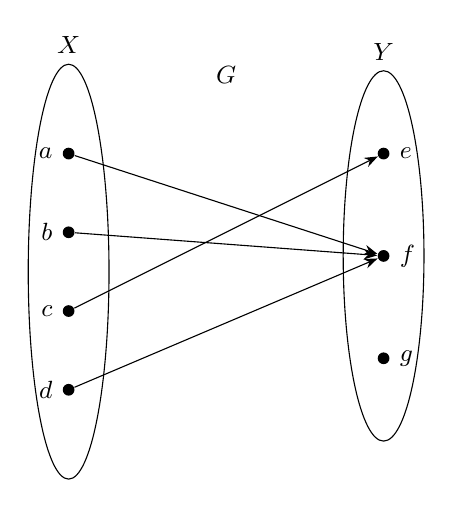
\begin{tikzpicture}[
    >=Stealth,
    dot/.style={circle, fill, inner sep=1.5pt},
    every node/.style={font=\small}
  ]
  % Domain
  \node[dot, label=left:{$a$}] (a) at (0,2.5) {};
  \node[dot, label=left:{$b$}] (b) at (0,1.5) {};
  \node[dot, label=left:{$c$}] (c) at (0,0.5) {};
  \node[dot, label=left:{$d$}] (d) at (0,-0.5){};
  \node[draw, ellipse, fit=(a)(b)(c)(d), inner sep=8pt, label=above:{$X$}] {};

  % Codomain
  \node[dot, label=right:{$e$}] (e) at (4,2.5) {};
  \node[dot, label=right:{$f$}] (f) at (4,1.2) {};
  \node[dot, label=right:{$g$}] (g) at (4,-0.1){};
  \node[draw, ellipse, fit=(e)(f)(g), inner sep=8pt, label=above:{$Y$}] {};

  % Arrows
  \draw[->] (a) -- (f);
  \draw[->] (b) -- (f);
  \draw[->] (c) -- (e);
  \draw[->] (d) -- (f);

  % Label
  \node at (2,3.5) {$G$};
\end{tikzpicture}
\end{center}

\noindent
Is $G$ one-to-one? Why or why not? Is $G$ onto? Why or why not?

\bigskip

%% ─────────────────────────────────────────────
\noindent\textbf{Problem 4} (Epp 7.2 \#8). \;
Let $X = \{a, b, c\}$ and $Y = \{d, e, f, g\}$.
Define functions $H$ and $K$ by the following arrow diagrams.

\begin{center}
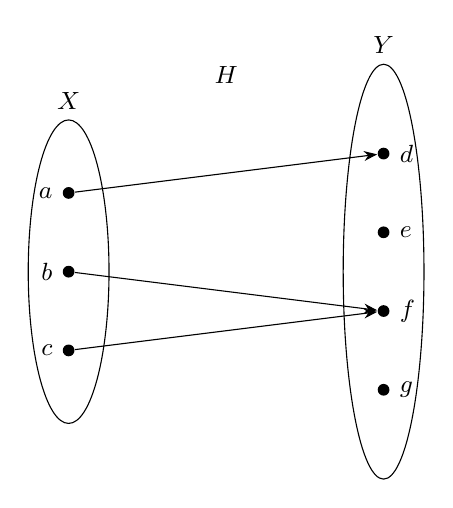
\begin{tikzpicture}[
    >=Stealth,
    dot/.style={circle, fill, inner sep=1.5pt},
    every node/.style={font=\small}
  ]
  % ---- H ----
  % Domain
  \node[dot, label=left:{$a$}] (ha) at (0,2)   {};
  \node[dot, label=left:{$b$}] (hb) at (0,1)   {};
  \node[dot, label=left:{$c$}] (hc) at (0,0)   {};
  \node[draw, ellipse, fit=(ha)(hb)(hc), inner sep=8pt, label=above:{$X$}] {};

  % Codomain
  \node[dot, label=right:{$d$}] (hd) at (4,2.5) {};
  \node[dot, label=right:{$e$}] (he) at (4,1.5) {};
  \node[dot, label=right:{$f$}] (hf) at (4,0.5) {};
  \node[dot, label=right:{$g$}] (hg) at (4,-0.5){};
  \node[draw, ellipse, fit=(hd)(he)(hf)(hg), inner sep=8pt, label=above:{$Y$}] {};

  % Arrows
  \draw[->] (ha) -- (hd);
  \draw[->] (hb) -- (hf);
  \draw[->] (hc) -- (hf);

  % Label
  \node at (2,3.5) {$H$};
\end{tikzpicture}
\hspace{1.5cm}
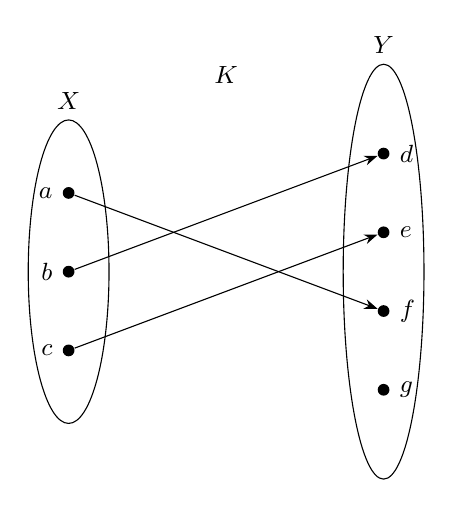
\begin{tikzpicture}[
    >=Stealth,
    dot/.style={circle, fill, inner sep=1.5pt},
    every node/.style={font=\small}
  ]
  % ---- K ----
  % Domain
  \node[dot, label=left:{$a$}] (ka) at (0,2)   {};
  \node[dot, label=left:{$b$}] (kb) at (0,1)   {};
  \node[dot, label=left:{$c$}] (kc) at (0,0)   {};
  \node[draw, ellipse, fit=(ka)(kb)(kc), inner sep=8pt, label=above:{$X$}] {};

  % Codomain
  \node[dot, label=right:{$d$}] (kd) at (4,2.5) {};
  \node[dot, label=right:{$e$}] (ke) at (4,1.5) {};
  \node[dot, label=right:{$f$}] (kf) at (4,0.5) {};
  \node[dot, label=right:{$g$}] (kg) at (4,-0.5){};
  \node[draw, ellipse, fit=(kd)(ke)(kf)(kg), inner sep=8pt, label=above:{$Y$}] {};

  % Arrows
  \draw[->] (ka) -- (kf);
  \draw[->] (kb) -- (kd);
  \draw[->] (kc) -- (ke);

  % Label
  \node at (2,3.5) {$K$};
\end{tikzpicture}
\end{center}

\begin{enumerate}[label=\alph*.]
  \item Is $H$ one-to-one? Why or why not? Is it onto? Why or why not?
  \item Is $K$ one-to-one? Why or why not? Is it onto? Why or why not?
\end{enumerate}

\bigskip

%% ─────────────────────────────────────────────
\noindent\textbf{Problem 5} (Epp 7.3 \#5). \;
Define $f \colon \R \to \R$ by the rule $f(x) = -x$ for every real number $x$.
Find $(f \circ f)(x)$.

\bigskip

%% ─────────────────────────────────────────────
\noindent\textbf{Problem 6} (Epp 7.3 \#11). \;
Define $F \colon \R \to \R$ and $G \colon \R \to \R$ by the rules
\[
  F(x) = 3x
  \qquad\text{and}\qquad
  G(x) = \left\lceil \frac{x}{3} \right\rceil
  \quad \text{for every real number } x.
\]

\begin{enumerate}[label=\alph*.]
  \item Find $(G \circ F)(6)$, $(F \circ G)(6)$, $(G \circ F)(1)$, and $(F \circ G)(1)$.
  \item Is $G \circ F = F \circ G$? Explain.
\end{enumerate}

\bigskip

%% ─────────────────────────────────────────────
\noindent\textbf{Problem 7}. \;
Let $f \colon X \to Y$ and $g \colon Y \to Z$.
Prove or disprove: if $g \circ f$ is bijective, then $f$ is bijective.

\end{document}
